\documentclass[10pt]{beamer}

\usetheme{CambridgeUS}
\setbeamercolor{titlelike}{bg=darkred}

\title{\color{white}Slides Progetto LAM 2023/2024}
\author{Matteo Canghiari}
\institute[Informatica per il Management]{Informatica per il Management \\ Università di Bologna}
\date{Gennaio 27, 2025}

\begin{document}

\frame{\titlepage}

\begin{frame}
\frametitle{Contents}
\tableofcontents
\end{frame}

\section{Scelte di base}
\begin{frame}{Scelte di base}
Nel corso dello sviluppo dell'applicazione sono state effettuate diverse scelte progettuali, quali:
\begin{itemize}
    \item Uso di Kotlin
    \item Design pattern architetturale MVVM
    \item Jetpack compose per animazioni durante runtime
    \item Supabase service come SSOT, di cui memorizzata una copia in locale
    \item Bucket di AWS per condivisione dei dati tra utenti iscritti all'applicazione
\end{itemize}
\end{frame}

\section{Divisione e struttura del codice}
\begin{frame}{Divisione e struttura del codice}
La suddivisione del progetto avviene in differenti componenti, ognuna delle quali è destinata nella propria sub-directory, suddivise in:
\begin{itemize}
    \item activity
    \item fragment
    \item page
    \item receiver
    \item room
    \item service
    \item singleton 
    \item viewModel
    \item worker
\end{itemize}
\end{frame}

\section{Features principali}
\begin{frame}{Registrazione \& Login}
    \begin{columns}
        \begin{column}{0.5\textwidth}
            \hspace*{100pt}
            \begin{itemize}
                \item \small \textbf{Prime schermate} visualizzabili all'avvio dell'applicazione
                \item \small Controllo di \textbf{connessione} persistente del dispositivo
                \item \small Check di \textbf{unicità} delle credenziali di accesso
                \item \small \textbf{Reindirizzamento} autonomo alla Home dell'applicazione qualora l'accesso sia stato già effettuato
            \end{itemize}
        \end{column}
        \begin{column}{0.5\textwidth}
            \begin{center}
                \fbox{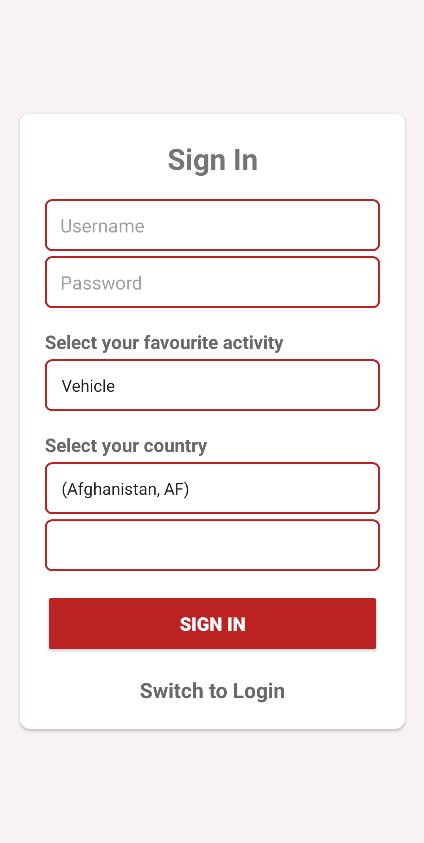
\includegraphics[width=72.5pt]{img/img1.png}}
                \fbox{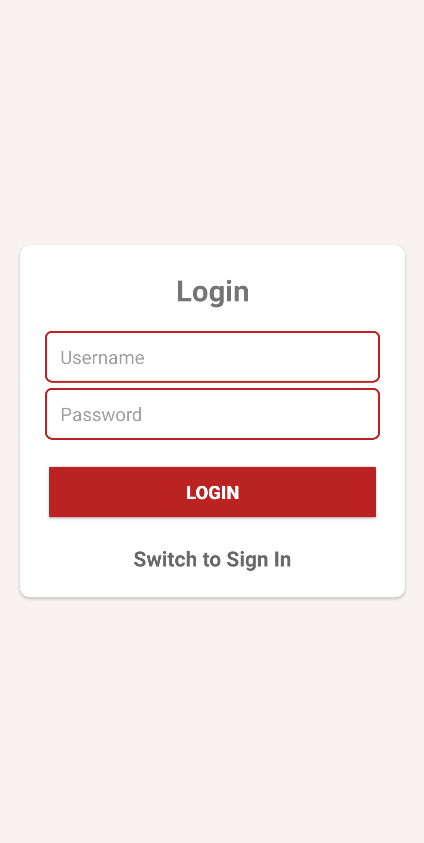
\includegraphics[width=72.5pt]{img/img2.png}}
            \end{center}
        \end{column}
    \end{columns}
\end{frame}

\begin{frame}{Home}
    \begin{columns}
        \begin{column}{0.5\textwidth}
            \hspace*{100pt}
            \begin{itemize}
                \item \small Visualizzazione della sezione personale tramite \textbf{TabLayout}
                \item \small \textbf{Progress page} ideata per evidenziare i progressi ottenuti durante la registrazione, manuale o autonoma, dell'attività motorie
                \item \small \textbf{Areas page} visualizzazione delle transizioni avvenute durante un certo arco temporale
            \end{itemize}
        \end{column}
        \begin{column}{0.5\textwidth}
            \begin{center}
                \fbox{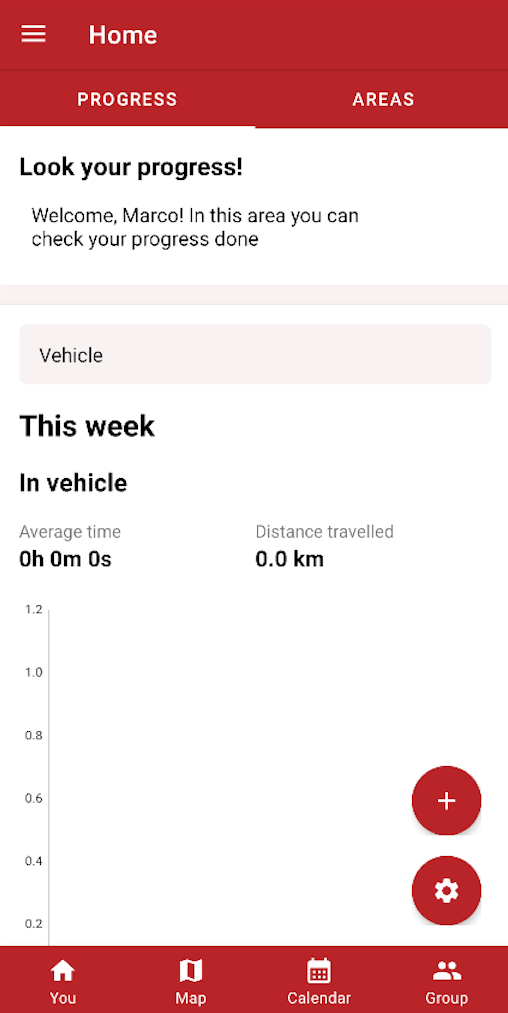
\includegraphics[width=72.5pt]{img/img3.png}}
                \fbox{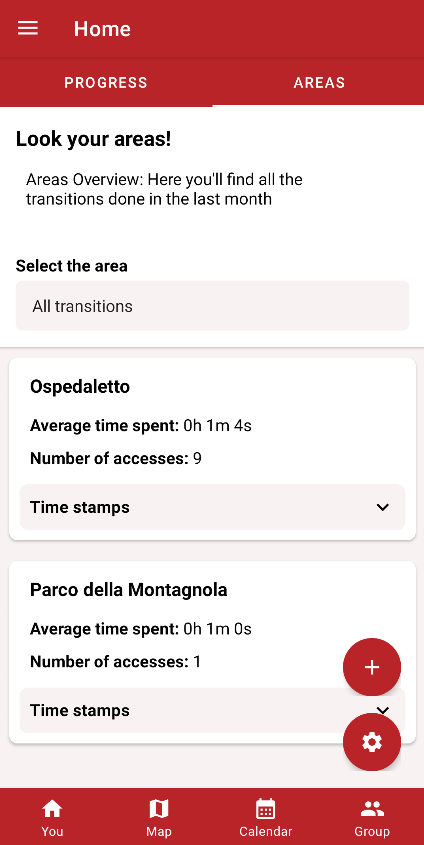
\includegraphics[width=72.5pt]{img/img4.png}}
            \end{center}
        \end{column}
    \end{columns}
\end{frame}

\begin{frame}{Map}
    \begin{columns}
        \begin{column}{0.5\textwidth}
            \hspace*{100pt}
            \begin{itemize}
                \item \small Mappa implementata tramite \textbf{Osmdroid} piuttosto che Google Maps
                \item \small Visualizzazione delle \textbf{aree geografiche} personali
                \item \small Aggiunta e rimozione delle aree geografiche tramite \textbf{SearchBar} e \textbf{Dialog}
                \item \small Floating button per marcare la \textbf{posizione corrente}
            \end{itemize}
        \end{column}
        \begin{column}{0.5\textwidth}
            \begin{center}
                \fbox{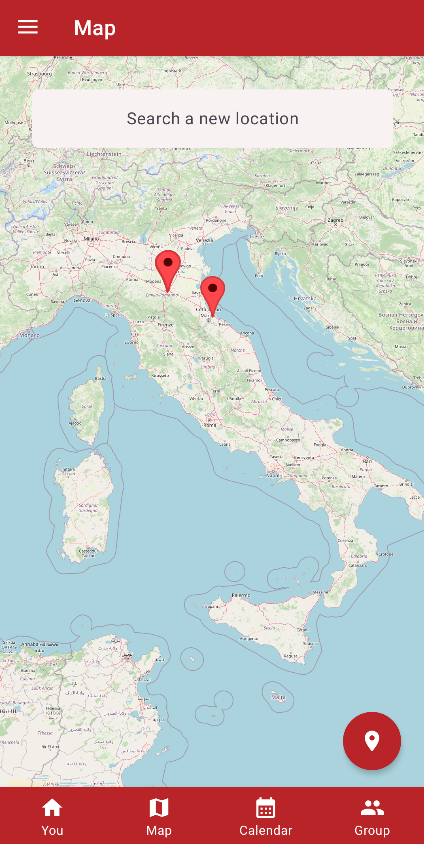
\includegraphics[width=72.5pt]{img/img5.png}}
                \fbox{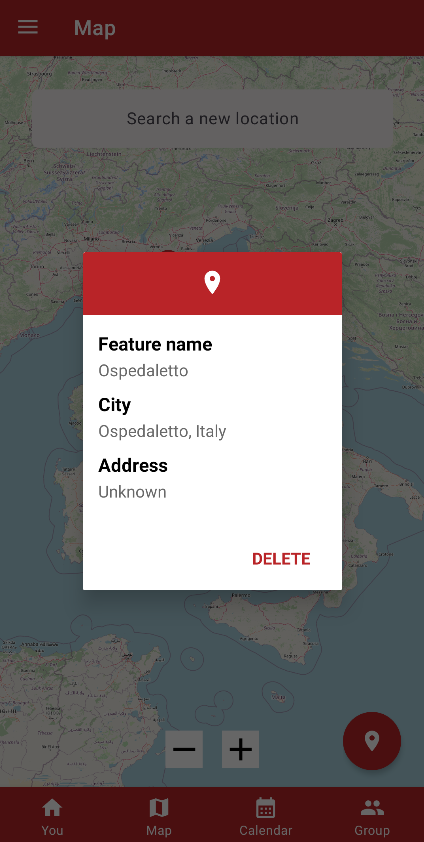
\includegraphics[width=72.5pt]{img/img6.png}}
            \end{center}
        \end{column}
    \end{columns}
\end{frame}

\begin{frame}{Calendar}
    \begin{columns}
        \begin{column}{0.5\textwidth}
            \hspace*{100pt}
            \begin{itemize}
                \item \small Visualizzazione schematica per l'organizzazione delle \textbf{proprie attività}
                \item \small Per ciascuna data selezionata sono mostrati tutti i \textbf{Memo} correnti
                \item \small Ciascun Memo può essere modificato oppure eliminato
                \item \small Tramite il floating button è garantito l'accesso al \textbf{form di creazione} di nuovi Memo
            \end{itemize}
        \end{column}
        \begin{column}{0.5\textwidth}
            \begin{center}
                \fbox{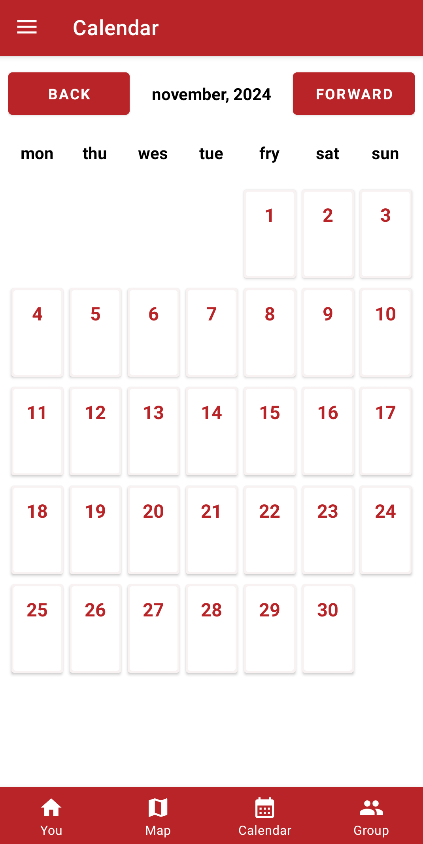
\includegraphics[width=72.5pt]{img/img7.png}}
                \fbox{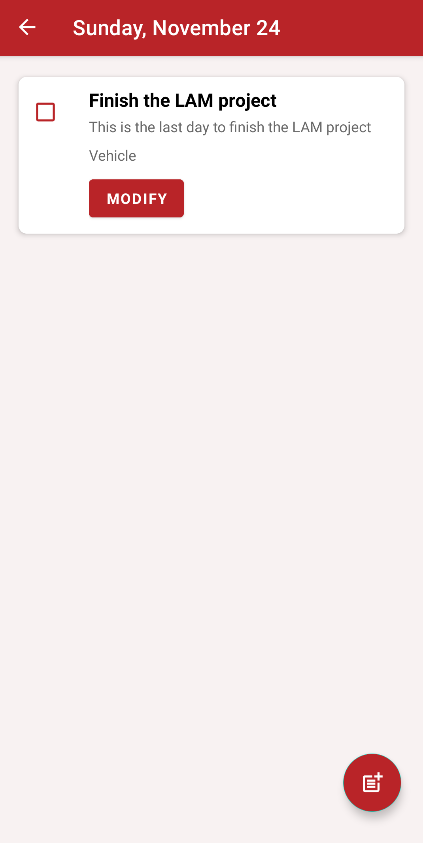
\includegraphics[width=72.5pt]{img/img8.png}}
            \end{center}
        \end{column}
    \end{columns}
\end{frame}

\begin{frame}{Group}
    \begin{columns}
        \begin{column}{0.5\textwidth}
            \hspace*{100pt}
            \begin{itemize}
                \item \small Accesso ai \textbf{dati condivisi} da parte di ulteriori iscritti
                \item \small Possibilità di cercare, aggiungere e rimuovere un utente oppure un amico
                \item \small Visualizzazione delle informazioni accessibili tramite \textbf{TabLayout}
            \end{itemize}
        \end{column}
        \begin{column}{0.5\textwidth}
            \begin{center}
                \fbox{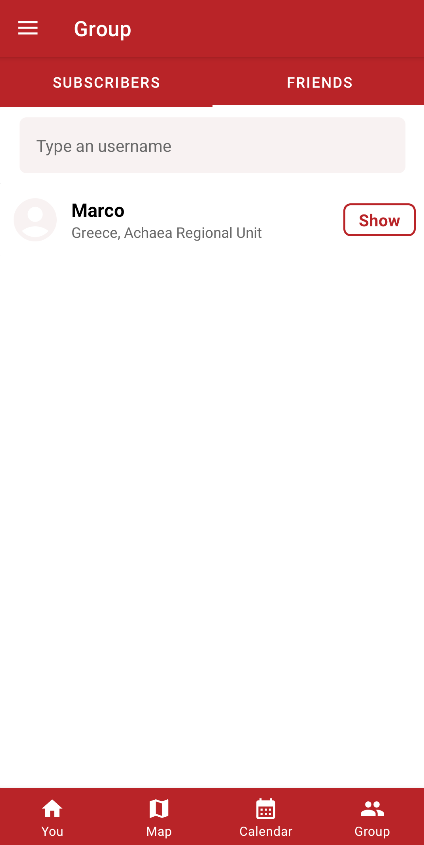
\includegraphics[width=72.5pt]{img/img9.png}}
                \fbox{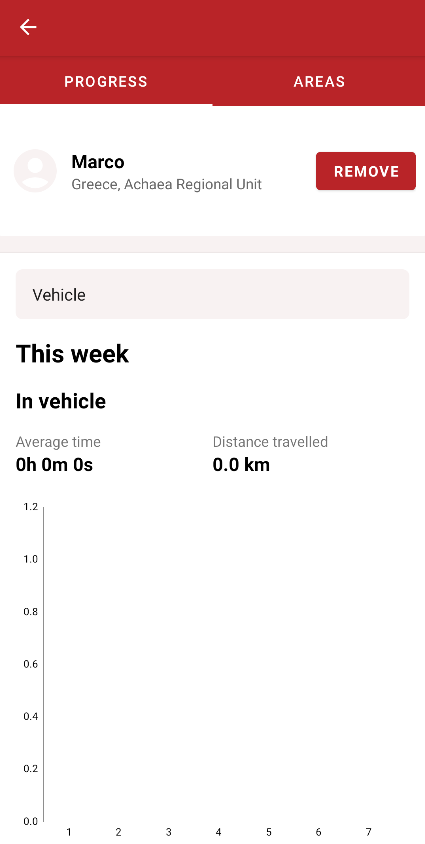
\includegraphics[width=72.5pt]{img/img10.png}}
            \end{center}
        \end{column}
    \end{columns}
\end{frame}

\begin{frame}{Settings}
    \begin{columns}
        \begin{column}{0.5\textwidth}
            \hspace*{100pt}
                \begin{itemize}
                    \item \small Centrallizzata la logica di \textbf{acquisizione dei permessi} durante il runtime
                    \item \small Pannello di controllo in cui l'utente può \textbf{abilitare e disabilitare} i servizi offerti
                    \item \small Definizione da parte dell'utente delle attività da monitorare tramite \textbf{Activity Recognition} 
                \end{itemize}
        \end{column}
        \begin{column}{0.5\textwidth}
            \begin{center}
                \fbox{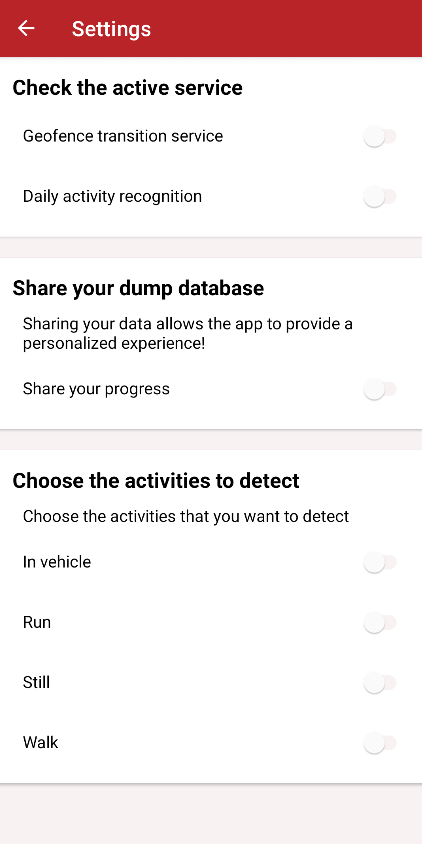
\includegraphics[width=72.5pt]{img/img13.png}}
            \end{center}
        \end{column}
    \end{columns}
\end{frame}

\section{Operazioni in background}
\begin{frame}{Operazioni in background}
    \small Le operazioni in background si articolano in tre sezioni differenti, quali:
    \begin{itemize}
        \item \small \textbf{Activity Recognition}, definizione e memorizzazione autonoma delle attività motorie compiute dall'utente
        \item \small \textbf{Geofencing}, memorizzazione delle transizioni dell'utente qualora dovesse varcare la soglia di un'area di interesse
        \item \small \textbf{Connectivity}, receiver utilizzato per acquisire tutti i cambiamenti incisivi di connessione del dispositivo
    \end{itemize}
\end{frame}

\begin{frame}{Architettura delle operazioni in background}
    \small A livello implementativo, tutte le background operations seguono una stessa architettura. Sono utilizzati tre componenti principali: Broadcast Receiver, Background Service e Worker. \vspace*{7pt}\\ Il Receiver è responsabile di intercettare gli intenti inviati dal SO, per poi delegare la manipolazione delle informazioni acquisite a specifici \textbf{Worker}. \vspace*{7pt}\\ I Worker provvederanno ad effettuare alcune operazioni di \textbf{pre-processing} prima di risvegliare i \textbf{Service}. \vspace*{7pt}\\ Infine, i Service, in base alle informazioni ricevute, stabileranno il comportamento successivo che debba mantenere l'applicazione.
\end{frame}

\section{SSOT}
\begin{frame}{SSOT}
    \small Il \textbf{Model} definisce l'insieme dei dati ritenuti autorevoli, memorizzati in un contenitore durante le interazioni con l'utente. Avviene una suddivisione del Model in due entità distinte, quali: Room e Supabase. \vspace*{7pt}\\ La decisione di sviluppare un doppio livello di persistenza dei dati nasce principalmente dall'esigenza di garantire che un singolo utente rimanga il punto di \textbf{riferimento unico} a livello locale. \vspace*{7pt}\\ Pertanto, il real time database è incaricato di memorizzare tutte le informazioni degli utenti iscritti. \vspace{7pt}\\ Al momento del login oppure del logout avviene un trasferimento dei dati secondo un formato consono, quale un dump, a seconda della casistica.
\end{frame}

\section{Bucker AWS}
\begin{frame}{Bucket AWS}
    \small La condivisione dei propri dati tramite l'applicazione avviene mediante \textbf{AWS}. \vspace*{7pt}\\ Abilitato il servizio all'interno dell'activity Settings, l'applicazione programmerà un \textbf{Worker periodico} incaricato di effettuare un \textbf{dump} del database. \vspace*{7pt}\\ Il dump è successivamente caricato all'interno di un \textbf{Bucket} mediante un richiesta \textbf{AWS-S3Client}.
\end{frame}
\end{document}